\documentclass[final]{article}
\PassOptionsToPackage{numbers}{natbib}

% Style and formatting packages
\usepackage{neurips_2024}
\usepackage[utf8]{inputenc} 
\usepackage[T1]{fontenc}    
\usepackage{graphicx}
\usepackage{booktabs}       
\usepackage{amsfonts}       
\usepackage{nicefrac}       
\usepackage{microtype}      
\usepackage{enumitem,amssymb}
\usepackage{xcolor}
\usepackage{hyperref}
\usepackage{url}

% Custom checklist
\newlist{todolist}{itemize}{2}
\setlist[todolist]{label=$\square$}

% Color setup
\definecolor{niceblue}{rgb}{0, 0.5, 1.0}
\definecolor{nicered}{rgb}{.617, .039, .031}
\hypersetup{colorlinks, linkcolor=niceblue, citecolor=niceblue, urlcolor=niceblue}

\title{Insurance Complaint Analysis using Machine Learning Methods}

\author{%
  Matthew Lucia \\
  University of Vermont\\
  Burlington, VT 05405 \\
  \texttt{mlucia@uvm.edu} \\
  \And
  Conor McDevitt \\
  University of Vermont \\
  Burlington, VT 05405 \\
  \texttt{cdmcdevi@uvm.edu} \\
  \And
  Ryan Courtney \\
  University of Vermont \\
  Burlington, VT 05405 \\
  \texttt{racourtn@uvm.edu} \\
}

\begin{document}

\maketitle

\begin{abstract}
Insurance companies receive many complaints regarding claim handling, policyholder service, underwriting issues, and more. Understanding the patterns in these complaints can help insurance providers improve their services, reduce disputes, and streamline resolution processes.

The primary objectives of our research include:
\begin{enumerate}
  \item Developing predictive models to understand complaint characteristics
  \item Creating embeddings to capture nuanced textual information
  \item Improving complaint resolution processes through intelligent analysis
\end{enumerate}
By building Neural Networks and Logistic Regression models with embeddings, we can extract meaningful features from complex complaint data, predict complaint dispositions and recovery amounts with higher accuracy, and provide insights into complaint patterns to assist insurance companies address issues.
\end{abstract}

\section{Introduction and Problem Definition}

Identifying common reasons for complaints can help insurance companies proactively address issues. Predicting complaint resolution time or recovery amount can assist in optimizing customer support, and analyzing complaint outcomes can provide insight into systemic inefficiencies.

\section{Related Work and Bibliography}

Since insurance claims are abundant and time-consuming to process, machine learning offers a promising solution. However, literature reflects no single agreed-upon approach. Text-heavy claims add complexity due to the subjectivity of language.

\begin{enumerate}
  \item Models should be explainable. Insurance involves significant financial stakes, and stakeholders want to understand the reasoning behind predictions. Logistic regression offers interpretability, unlike some neural methods.
  \item Gilpin et al. (2018) propose heuristic techniques including: 
  \begin{itemize}
    \item Local model-agnostic explanations (e.g., LIME, SHAP)
    \item Visualization tools such as partial dependence plots and ICE plots
  \end{itemize}
\end{enumerate}

\section{Model and Training Algorithm}

\begin{enumerate}
  \item \textbf{Inputs}
    \begin{itemize}
      \item Categorical: Coverage, SubCoverage, Reason, SubReason, Status
      \item Numerical: Complaint duration, Recovery amount
      \item Text: Conclusion Statement
    \end{itemize}
  \item \textbf{Model Architecture}
    \begin{itemize}
      \item Text Embeddings: Pre-trained (e.g., Word2Vec)
      \item Neural Network: Embeddings $\rightarrow$ dense layers $\rightarrow$ softmax
      \item Logistic Regression with embeddings and L1/L2 regularization
    \end{itemize}
  \item \textbf{Outputs}
    \begin{itemize}
      \item Classification: Complaint reason, disposition
      \item Regression: Recovery amount, resolution time
    \end{itemize}
\end{enumerate}

\begin{figure}[h]
  \centering
  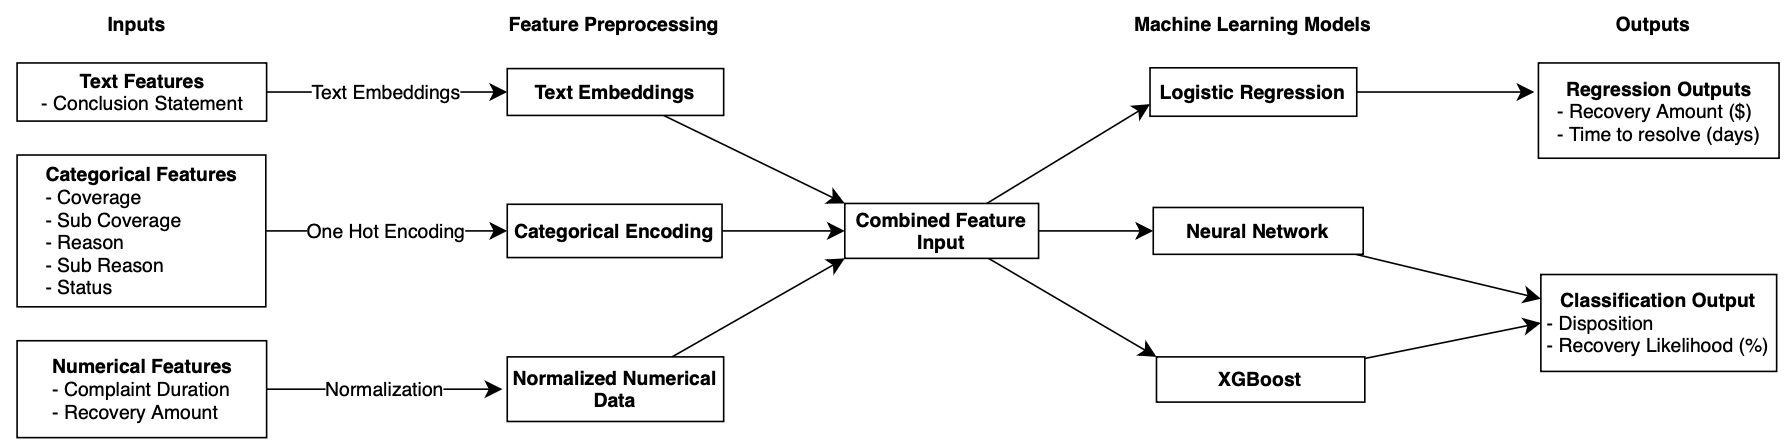
\includegraphics[width=1.0\textwidth]{ml-flowchart.png}
  \caption{Pipeline}
  \label{fig: Pipeline}
\end{figure}

\section{Dataset}

\subsection{Data Source}
“Insurance Company Complaints” dataset from Kaggle. Public dataset of consumer complaints filed in Connecticut.

\subsection{Dimensions}
\begin{itemize}
  \item 32,267 rows, 12 columns
\end{itemize}

\subsection{Data Preprocessing}
\begin{itemize}
  \item Remove incomplete rows/columns
  \item Derived features:
  \begin{itemize}
    \item Complaint duration: Days between 'Closed' and 'Opened'
    \item Text embeddings
  \end{itemize}
  \item Normalize numerical features
  \item Encode categorical variables
\end{itemize}

\subsection{Embedding Strategy}
Pre-trained embeddings (Word2Vec, GloVe) to represent text features semantically.

\section{Experimental Evaluation}

\subsection{Evaluation Methodology}
\begin{itemize}
  \item 70\% train / 20\% test / 10\% validation split
\end{itemize}

\subsection{Results}
To be completed.

\subsection{Discussion}
To be completed.

\section{Conclusion}
To be completed.

\bibliographystyle{plainnat}
\bibliography{references}

% Add actual entries to references.bib or inline here
% Example inline references:
\begin{thebibliography}{9}

\bibitem{johnson2023}
Johnson, M., Albizri, A., \& Harfouche, A. (2023).
Responsible Artificial Intelligence in Healthcare: Predicting and Preventing Insurance Claim Denials.
\textit{Information Systems Frontiers}, 25, 2179–2195. \url{https://doi.org/10.1007/s10796-021-10137-5}

\bibitem{gilpin2018}
Gilpin, L. H., Bau, D., Yuan, B. Z., Bajwa, A., Specter, M., \& Kagal, L. (2018).
Explaining explanations: An approach to evaluating interpretability of machine learning.

\end{thebibliography}

\end{document}